%&"../../visual"
\endofdump
\geometry{
    right=0.45\paperwidth,
    marginparwidth=0.4\paperwidth
}
\begin{document}
    \title{酒店数据交互分析}
    \maketitle

    \marginpar{
        \begin{figure}[H]
            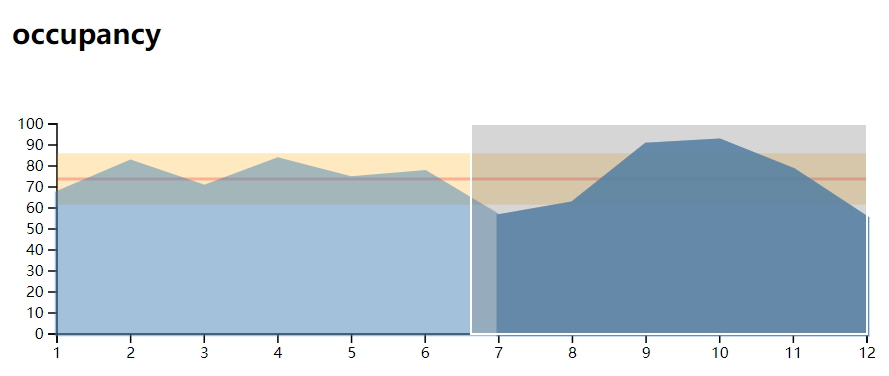
\includegraphics[width=\linewidth]{occupancy}
            \caption{占有率折线图}\label{fig:pccupancy}
        \end{figure}
    }

    \section{问题一}

    \paragraph{问题} 找到酒店淡季、旺季的时间段。

    \paragraph{方法} 使用折线面积图展现 \verb"occupancy" 字段的数据,并采取 \verb"brush" 筛选数据范围,以与后面的图形联动。

    \paragraph{结论} 认为基本小于 $\mu-\sigma$ 的月份:7, 8, 12 月为淡季;大于 $\mu+\sigma$ 的月份:9, 10 月为旺季。

    \marginpar{
        \begin{figure}[H]
            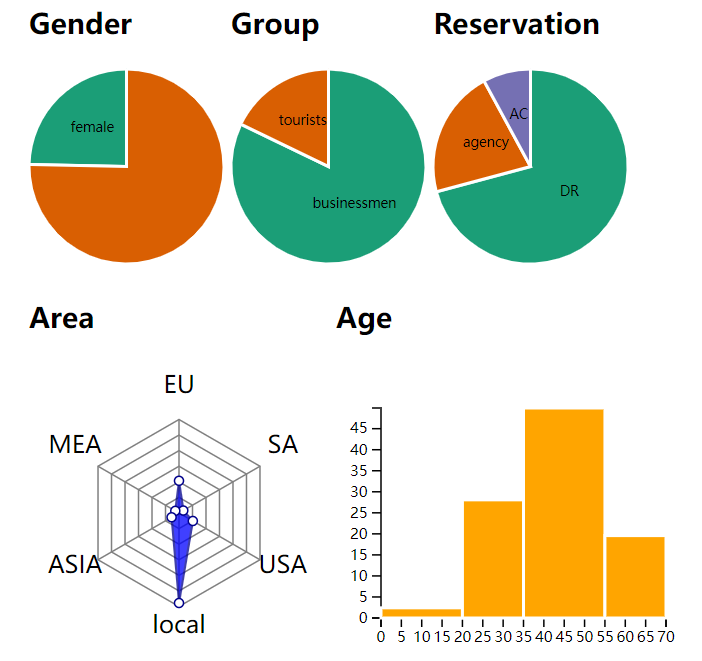
\includegraphics[width=\linewidth]{chara}
            \caption{入住人员特点}\label{fig:chara}
        \end{figure}
    }

    \section{问题二}

    \paragraph{问题} 分析酒店入住人员的特点,尝试回答:酒店住客有什么特征?12 个月中住客特点是否发生过变化?如果是,分析哪些因素可能导致了变化。

    \paragraph{方法 (1)} 特征包括性别 \verb"female"(饼图呈现),源地 \verb"local", \verb"USA", \verb"SA", \verb"EU", \verb"MEA", \verb"ASIA"(雷达图呈现),商旅 \verb"businessmen", \verb"tourists"(饼图呈现),预约类型 \verb"DR", \verb"agenecy", \verb"AC"(饼图呈现),年龄分布 \verb"u20", \verb"20to35", \verb"35to55", \verb"m55"(直方图呈现)。数据将会取范围平均值。

    \paragraph{结论 (1)} 性别方面,男生较多;组别方面,商人居多;预约方式上,直接预约居多;地域方面,本地人居多;年龄组成上,35--55 岁的居多。

    \paragraph{方法 (2)} 为了验证 12 个月趋势,采用平行坐标图来观察这些变量的分布是否一致,如果不一致,则按照不同的因素分类线,观察坐标轴上颜色的杂乱程度。

    \paragraph{结论 (2)} 

    \marginpar{
        \begin{figure}[H]
            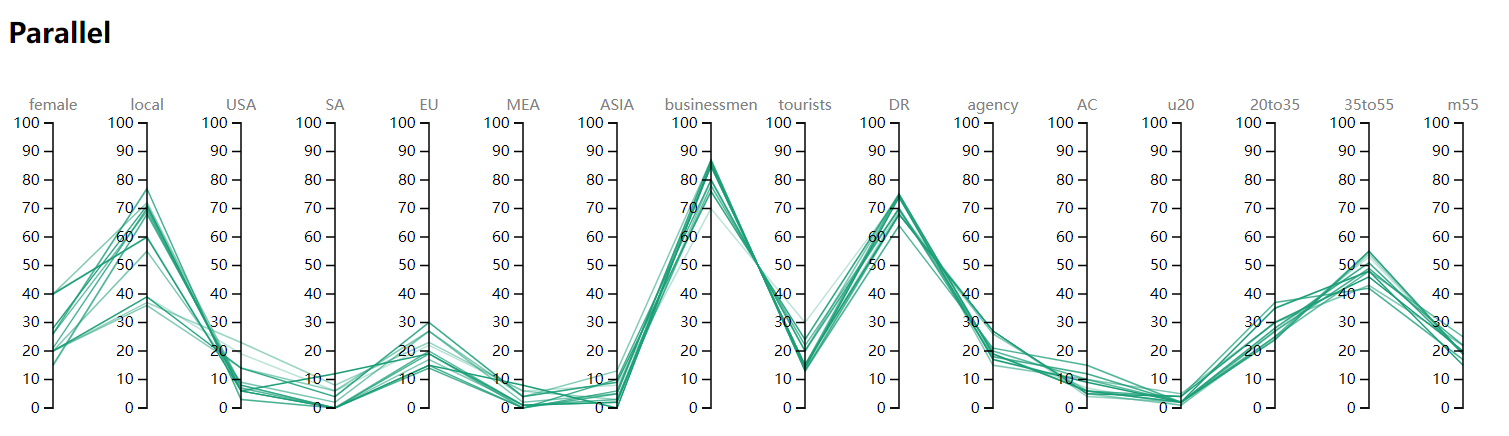
\includegraphics[width=\linewidth]{parallel}
            \caption{特点平行图}\label{fig:parallel}
        \end{figure}
    }

    大部分特点发生了 10\% -- 20\% 的变化,其中性别和地域变化较为明显。通过图 \ref{fig:seasonal} 中的图例控制颜色分类方法,进一步的实验表明,\verb"price", \verb"occupancy" 等因素对从 \verb"businessmen" 之后的列分类效果较好,颜色有规律地排列:价格越高或占有率越大(旺季),商人比重越高,35--55 岁人越多。而对于性别和地域方面,需要通过问题 \ref{sec:four} 的进一步讨论。

    \section{问题三}

    \marginpar{
        \begin{figure}[H]
            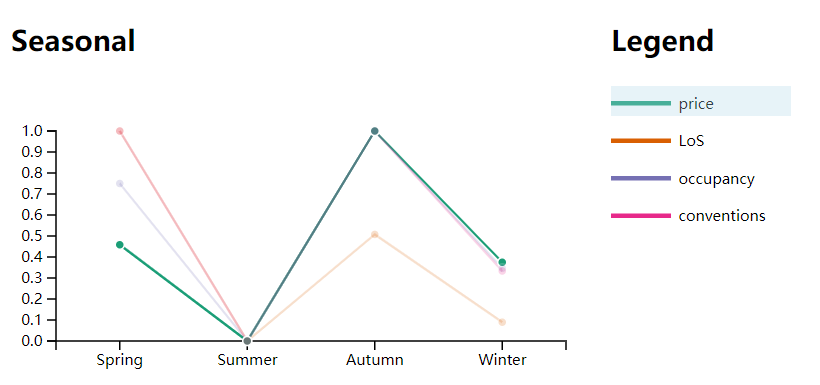
\includegraphics[width=\linewidth]{seasonal}
            \caption{季节折线图}\label{fig:seasonal}
        \end{figure}
    }

    \paragraph{问题} 分析\textbf{季节}因素对酒店的影响。并分析哪些因素有具有相似的季节性变化规律。

    \paragraph{方法} 主要考察 \verb"price", \verb"LoS", \verb"occupancy" 和\\ \verb"conventions" 这些因素在季节上的影响。将展示包含选中的完整季节的季节平均值折线图。

    \paragraph{结论} 夏季为淡季,秋季为旺季,春冬为平季。价格、入住时间和事件因素都具有相同的季节性变化规律。

    \marginpar{
        \begin{figure}[H]
            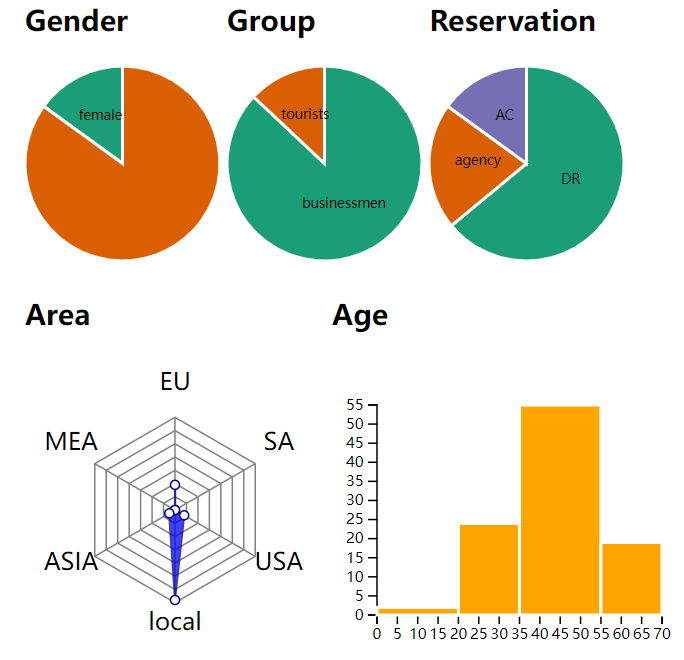
\includegraphics[width=\linewidth]{chara2}
            \caption{女性少的情形}\label{fig:chara2}
        \end{figure}
    }

    \section{问题四}\label{sec:four}

    \paragraph{问题} 除了以上问题外,写出自己分析过程中得到的其他结论。
    
    \paragraph{结论} 通过滑块筛选感知到,旺季时间本地人居多,将图 \ref{fig:chara2} 和图 \ref{fig:chara} 相对比,年轻人越多,女性越多。

    非常感谢表严肃的系列课程,让我充分理解了 JavaScript 设计模式 \cite{biao}。

    \bibliography{ref}

\end{document}